\chapter{Hardware vs Software}

In the preceding weeks we've learned about hardware, the physical components that make up computing
systems. Hardware is only half of what constitute computing systems. Software is the ``brain'' of
a computer system that dictates how the hardware should execute. Hardware without software is like
a car without a driver --- it is unable to do much. Similarly, software without hardware to run on
is like a driver without a car, it has nothing to drive. Together software and hardware are able to
perform work in a meaningful and controlled way.

In this section, we will discuss the distinction between hardware and software and how they
interact. As seen in Figure~\ref{fig:hw_sw:layers}, many layers of software sit between the hardware of
our computer systems and the software we use and develop. These layers build up from the hardware and
abstract away many of the complexities of lower levels to provide more and more functionality.

\begin{figure}
\centering
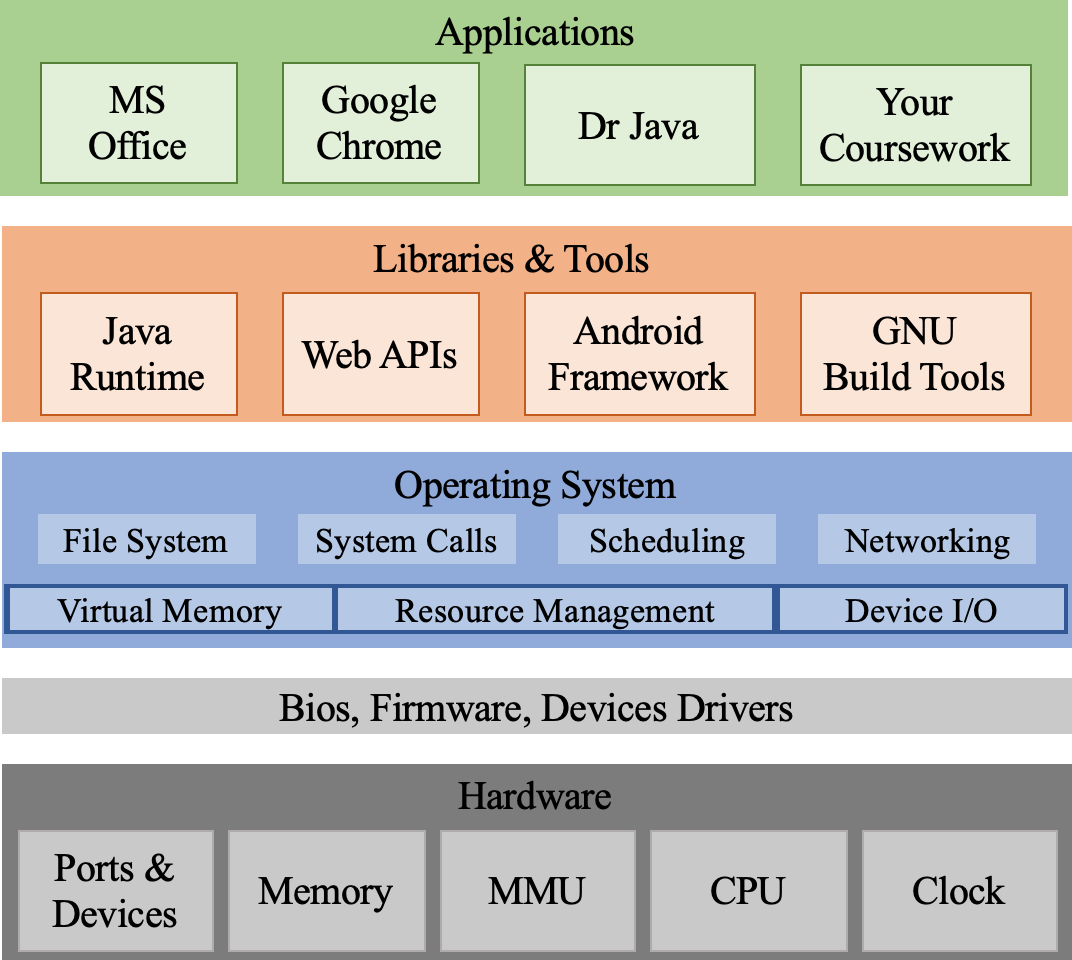
\includegraphics[width=6.5cm]{images/software_layers.png}
\caption{Layers of software built up from hardware. Each providing more abstractions and functionality for higher levels to use.}
\label{fig:hw_sw:layers}
\end{figure}

\section{Hardware}


\section{BIOS and Firmware}

\section{Operating Systems}

\section{Libraries and Tools}

\section{Applications}
